\chapter{EM}

\subsection{Dati geometrici}
\begin{center}
\begin{tabular}{|c|c|c|c|c|c|c|c|}
\midrule
\textit{Solenoide} & $n$ & $diametro_{int}$ & $diametro_{ext}$ & $diametro_{medio}$ & $l_{circonferenza}$ & $h$ & $A_{sezione}$  \\
		   & 322 & 0,05	 & 0,0937  & 0,0718 & 0,451 & 0,0225 &	0,000983 \\
 \midrule
\end{tabular}
\end{center}


\begin{center}
\begin{tabular}{|c|c|c|c|c|}
\midrule
\textit{Capacità} & $R_{int}$ (cm) & $R_{ext}$ (cm) & $lunghezza$ (cm) & $spessore piastre$ (cm)\\
   & 3.58 & 4.18  & 40  & 0.31 \\

 \midrule
\end{tabular}
\end{center}


Misuriamo c dalla relazione:
\begin{equation}
 c=\frac{1}{\sqrt{LC}}
\end{equation}
pertanto misuriamo la frequenza di risonanza di un cicuito RLC, per differenti configurazioni del circuito.

\subparagraph*{C ed L}
Nella prima parte dell'esperienza abbiamo verificato che i valori di capacità ed induttanza calcolati a partire dai parametri geometrici corrispondessero effettivamente a quelli misurati in laboratorio. 
Per tanto, in entrambi i circuiti, calcoliamo algebricamente i valori di V e $V_{0}$ per cui $t = \tau$. Inseriamo tali valori e misuriamo i tempo di scarica. Dalla stima del tempo caratteristico ricaviamo L e C. La capacità risulta in accordo, ed è stimata intorno ai $4.38$ nF, l'induttanza invece risulta:

\begin{center}
\begin{tabular}{c c}
$L_{geometrico}$  & 0.000293\\
$L_{misurato}$ & 0.000325\\
\end{tabular}
\end{center}

Visto che è presente una discrepanza tra i valori misurati e quelli geometrici, dovuto a capacità parassite, d'ora in avanti lavoreremo con una induttanza equivalente (modificando un parametro geometrico per ottenere l'accordo): $N_{eq} = 339$


\begin{comment}
Costruiamo un circuito RLC. Nota: il condensatore risente molto delle fluttuazioni, per cui lo colleghiamo a terra, per ridurle il più possibile.

Frequenze di risonanza intorno ai 500 kH (nota: è un minimo -> potenziale ai capi di LC)
\end{comment}


\subparagraph*{l=40 cm}

\begin{sagesilent}

 #Fit per stimare i parametri -> Frequenza di risonanza: -b/2a

#Carico file
raw = np.recfromcsv('dati/EM/40.csv')

#Seleziono dati per il fit
batch1 = raw[raw['freq']>640]
batch2 = batch1[batch1['freq']< 695]

#Carico negli array i dati giusti
freq = batch2['freq']
volt = batch2['vout']
yerr = batch2['errv']


def funz(x,a,b,c):
    return a*x^2+b*x+c

def func(P,x):
    return funz(x,P[0],P[1],P[2])

mymod = odr.Model(func)
mydata = odr.RealData(freq,volt)
myfit = odr.ODR(mydata,mymod,beta0=[1.,1.,1.],maxit=1000)
myout = myfit.run()

plt.clf()
xin = np.arange(min(freq)-10,max(freq)+10,1)
yin = func(myout.beta,xin)
plt.plot(freq,volt,'ro')
plt.errorbar(freq,volt,yerr,np.zeros_like(yerr),fmt=None)
plt.plot(xin,yin,'b--')
plt.grid(True)

#trovo minimo dai parametri x=-b/2*a
min1 = -myout.beta[1]/(2*myout.beta[0]) 

#stampo minimo su grafico
s = repr(round(min1,2))+" $(KHz)$"
plt.text(675,1.00,s,fontsize=12,bbox=dict(facecolor='red',alpha=0.1))

plt.savefig("grafici/EM/40.png",dpi=300)
 
\end{sagesilent}

\includegraphics[scale=0.75]{grafici/EM/40.png}




\subparagraph*{l=38 cm}

\begin{sagesilent}
#Fit per stimare i parametri -> Frequenza di risonanza: -b/2a

#Carico file
raw = np.recfromcsv('dati/EM/par38.csv')

#Seleziono dati per il fit
batch1 = raw[raw['freq']>675]
batch2 = batch1[batch1['freq']< 695]

#Carico negli array i dati giusti
freq = batch2['freq']
volt = batch2['vout']
yerr = batch2['errv']


def funz(x,a,b,c):
    return a*x^2+b*x+c

def func(P,x):
    return funz(x,P[0],P[1],P[2])

mymod = odr.Model(func)
mydata = odr.RealData(freq,volt)
myfit = odr.ODR(mydata,mymod,beta0=[1.,1.,1.],maxit=1000)
myout = myfit.run()

plt.clf()
xin = np.arange(min(freq)-10,max(freq)+10,1)
yin = func(myout.beta,xin)
plt.plot(freq,volt,'ro')
plt.errorbar(freq,volt,yerr,np.zeros_like(yerr),fmt=None)
plt.plot(xin,yin,'b--')
plt.grid(True)

#trovo minimo dai parametri x=-b/2*a
min2 = -myout.beta[1]/(2*myout.beta[0]) 

#stampo minimo su grafico
s = repr(round(min2,2))+" $(KHz)$"
plt.text(685,1.00,s,fontsize=12,bbox=dict(facecolor='red',alpha=0.1))

plt.savefig("grafici/EM/38.png",dpi=300)

\end{sagesilent}

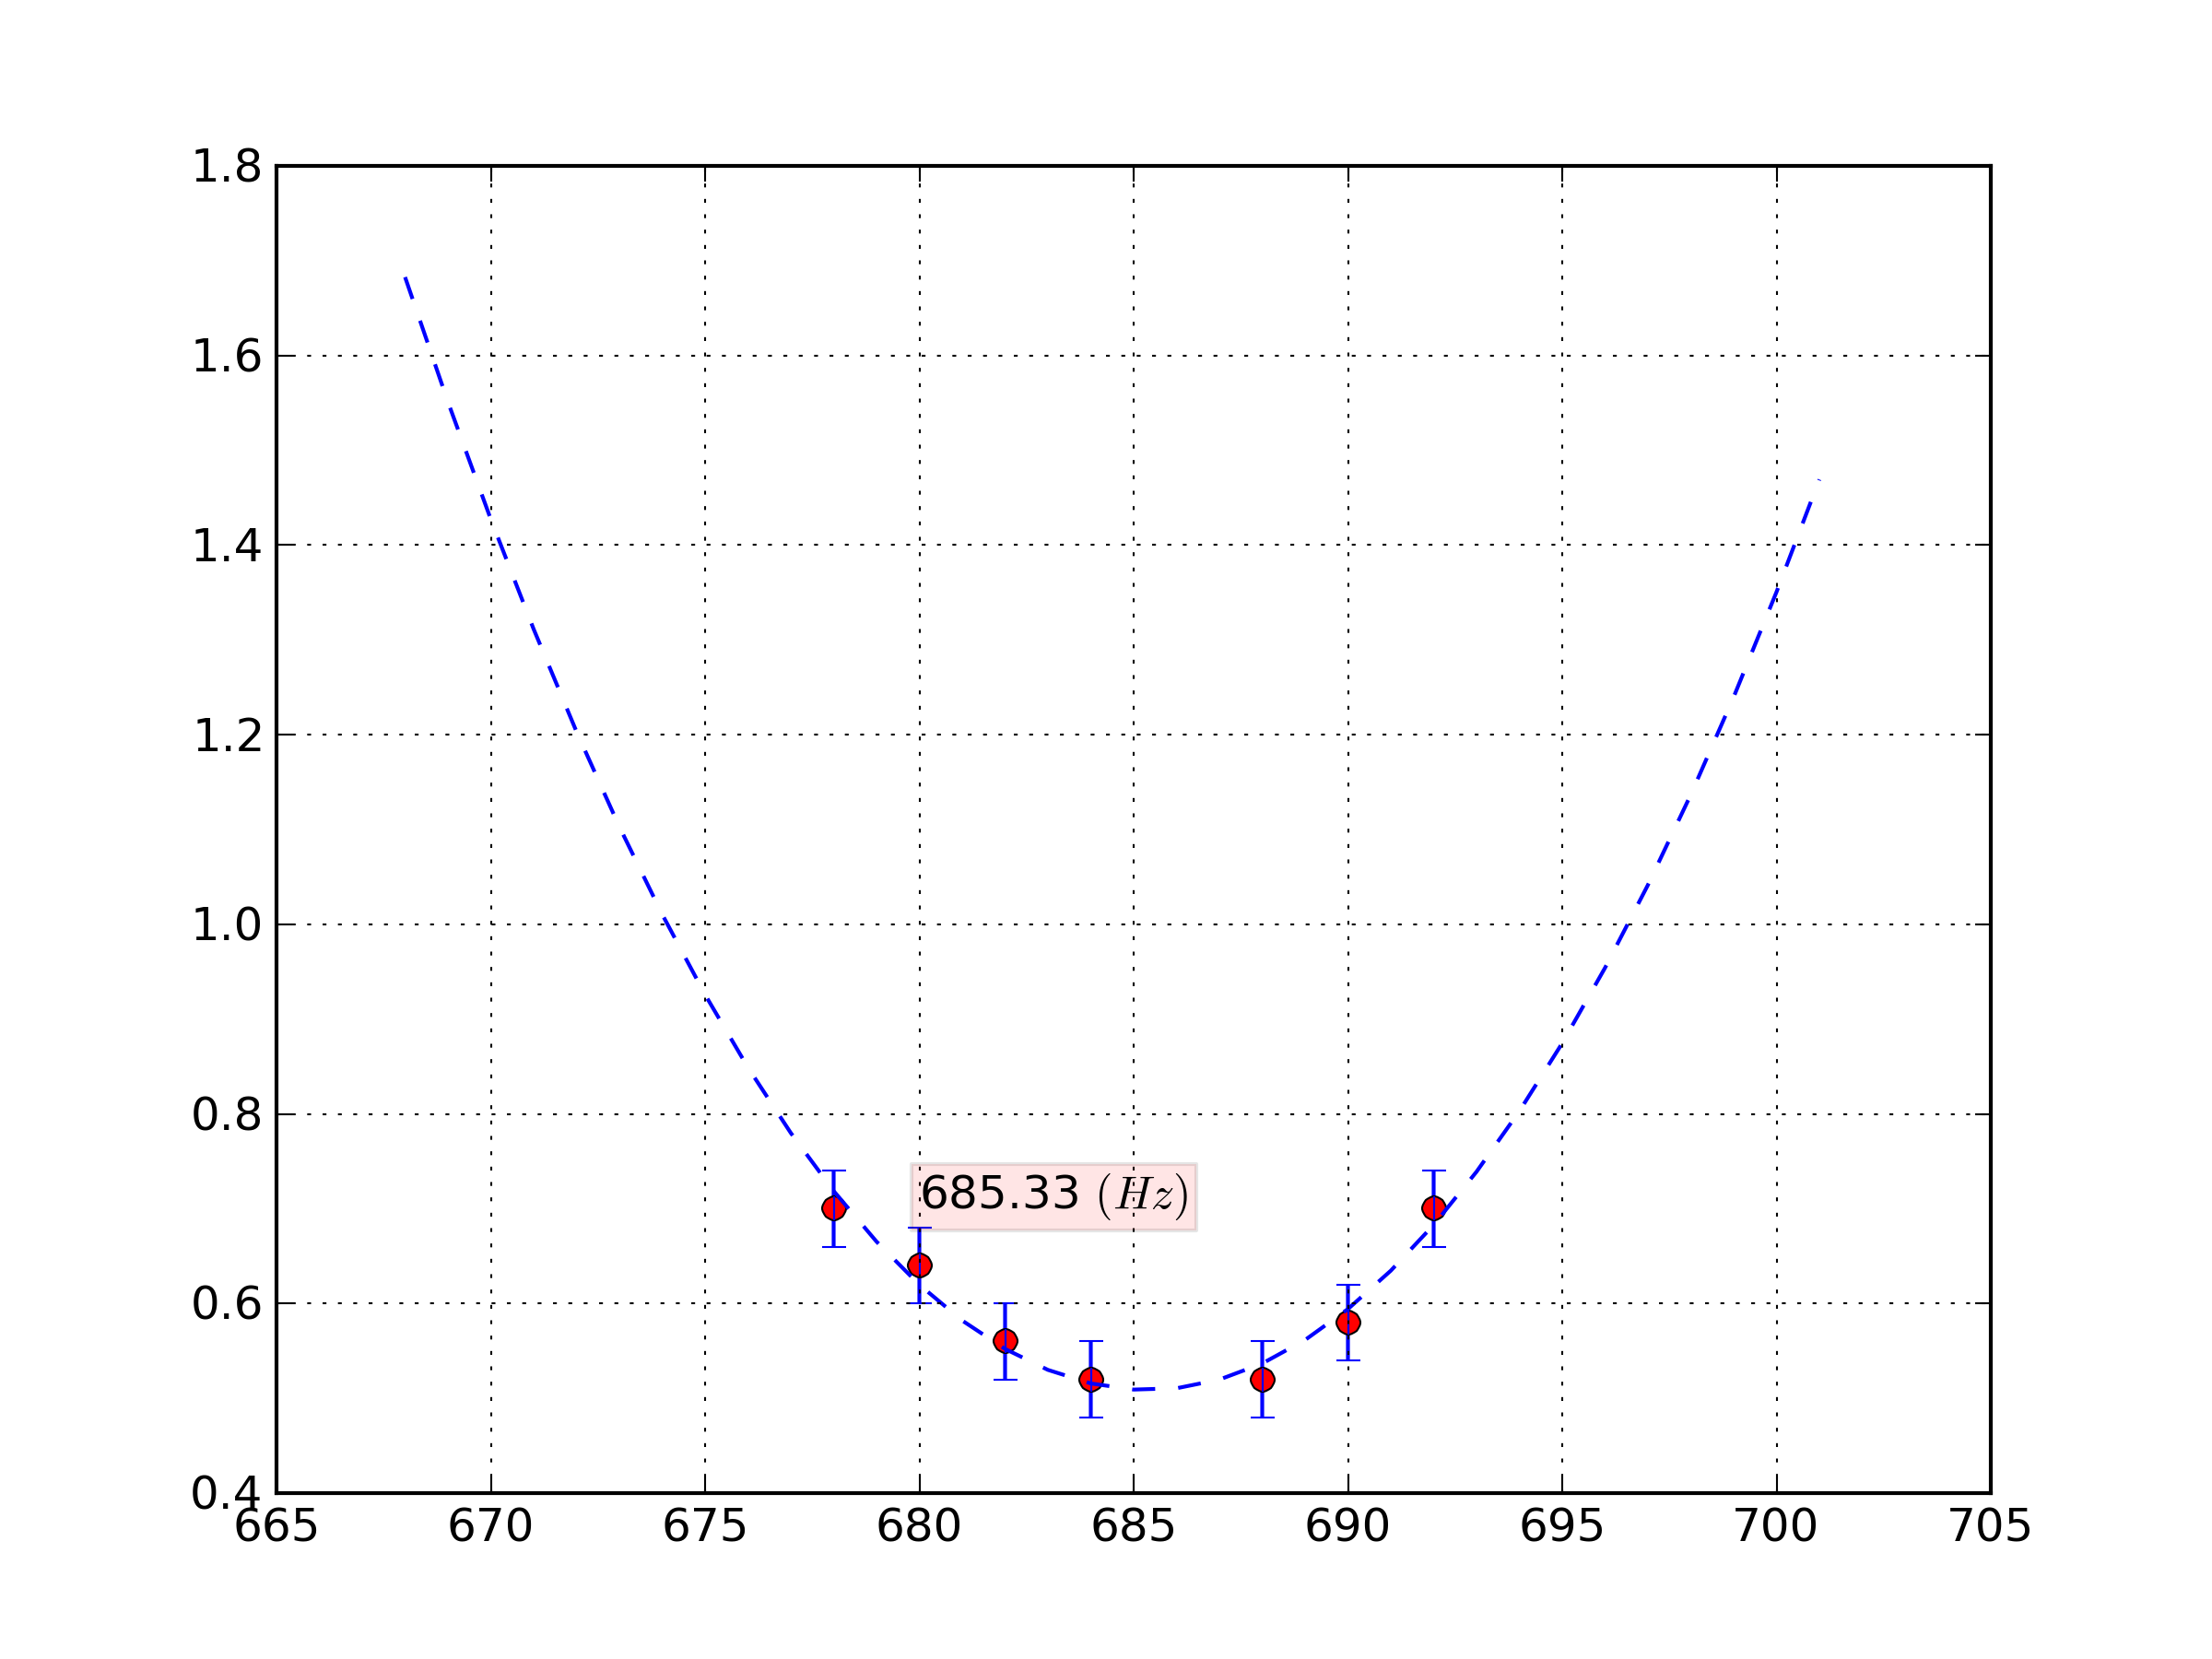
\includegraphics[scale=0.75]{grafici/EM/38.png}

\subparagraph*{l=34 cm}

\begin{sagesilent}
 #Fit per stimare i parametri -> Frequenza di risonanza: -b/2a

#Carico file
raw = np.recfromcsv('dati/EM/par34.csv')

#Seleziono dati per il fit
batch1 = raw[raw['freq']>680]
batch2 = batch1[batch1['freq']< 760]

#Carico negli array i dati giusti
freq = batch2['freq']
volt = batch2['vout']
yerr = batch2['errv']


def funz(x,a,b,c):
    return a*x^2+b*x+c

def func(P,x):
    return funz(x,P[0],P[1],P[2])

mymod = odr.Model(func)
mydata = odr.RealData(freq,volt)
myfit = odr.ODR(mydata,mymod,beta0=[1.,1.,1.],maxit=1000)
myout = myfit.run()

plt.clf()
xin = np.arange(min(freq)-10,max(freq)+10,1)
yin = func(myout.beta,xin)
plt.plot(freq,volt,'ro')
plt.errorbar(freq,volt,yerr,np.zeros_like(yerr),fmt=None)
plt.plot(xin,yin,'b--')
plt.grid(True)

#trovo minimo dai parametri x=-b/2*a
min3 = -myout.beta[1]/(2*myout.beta[0])


#stampo minimo su grafico
s = repr(round(min3,2))+" $(KHz)$"
plt.text(715,1.5,s,fontsize=12,bbox=dict(facecolor='red',alpha=0.1))

plt.savefig("grafici/EM/34.png",dpi=300)
\end{sagesilent}

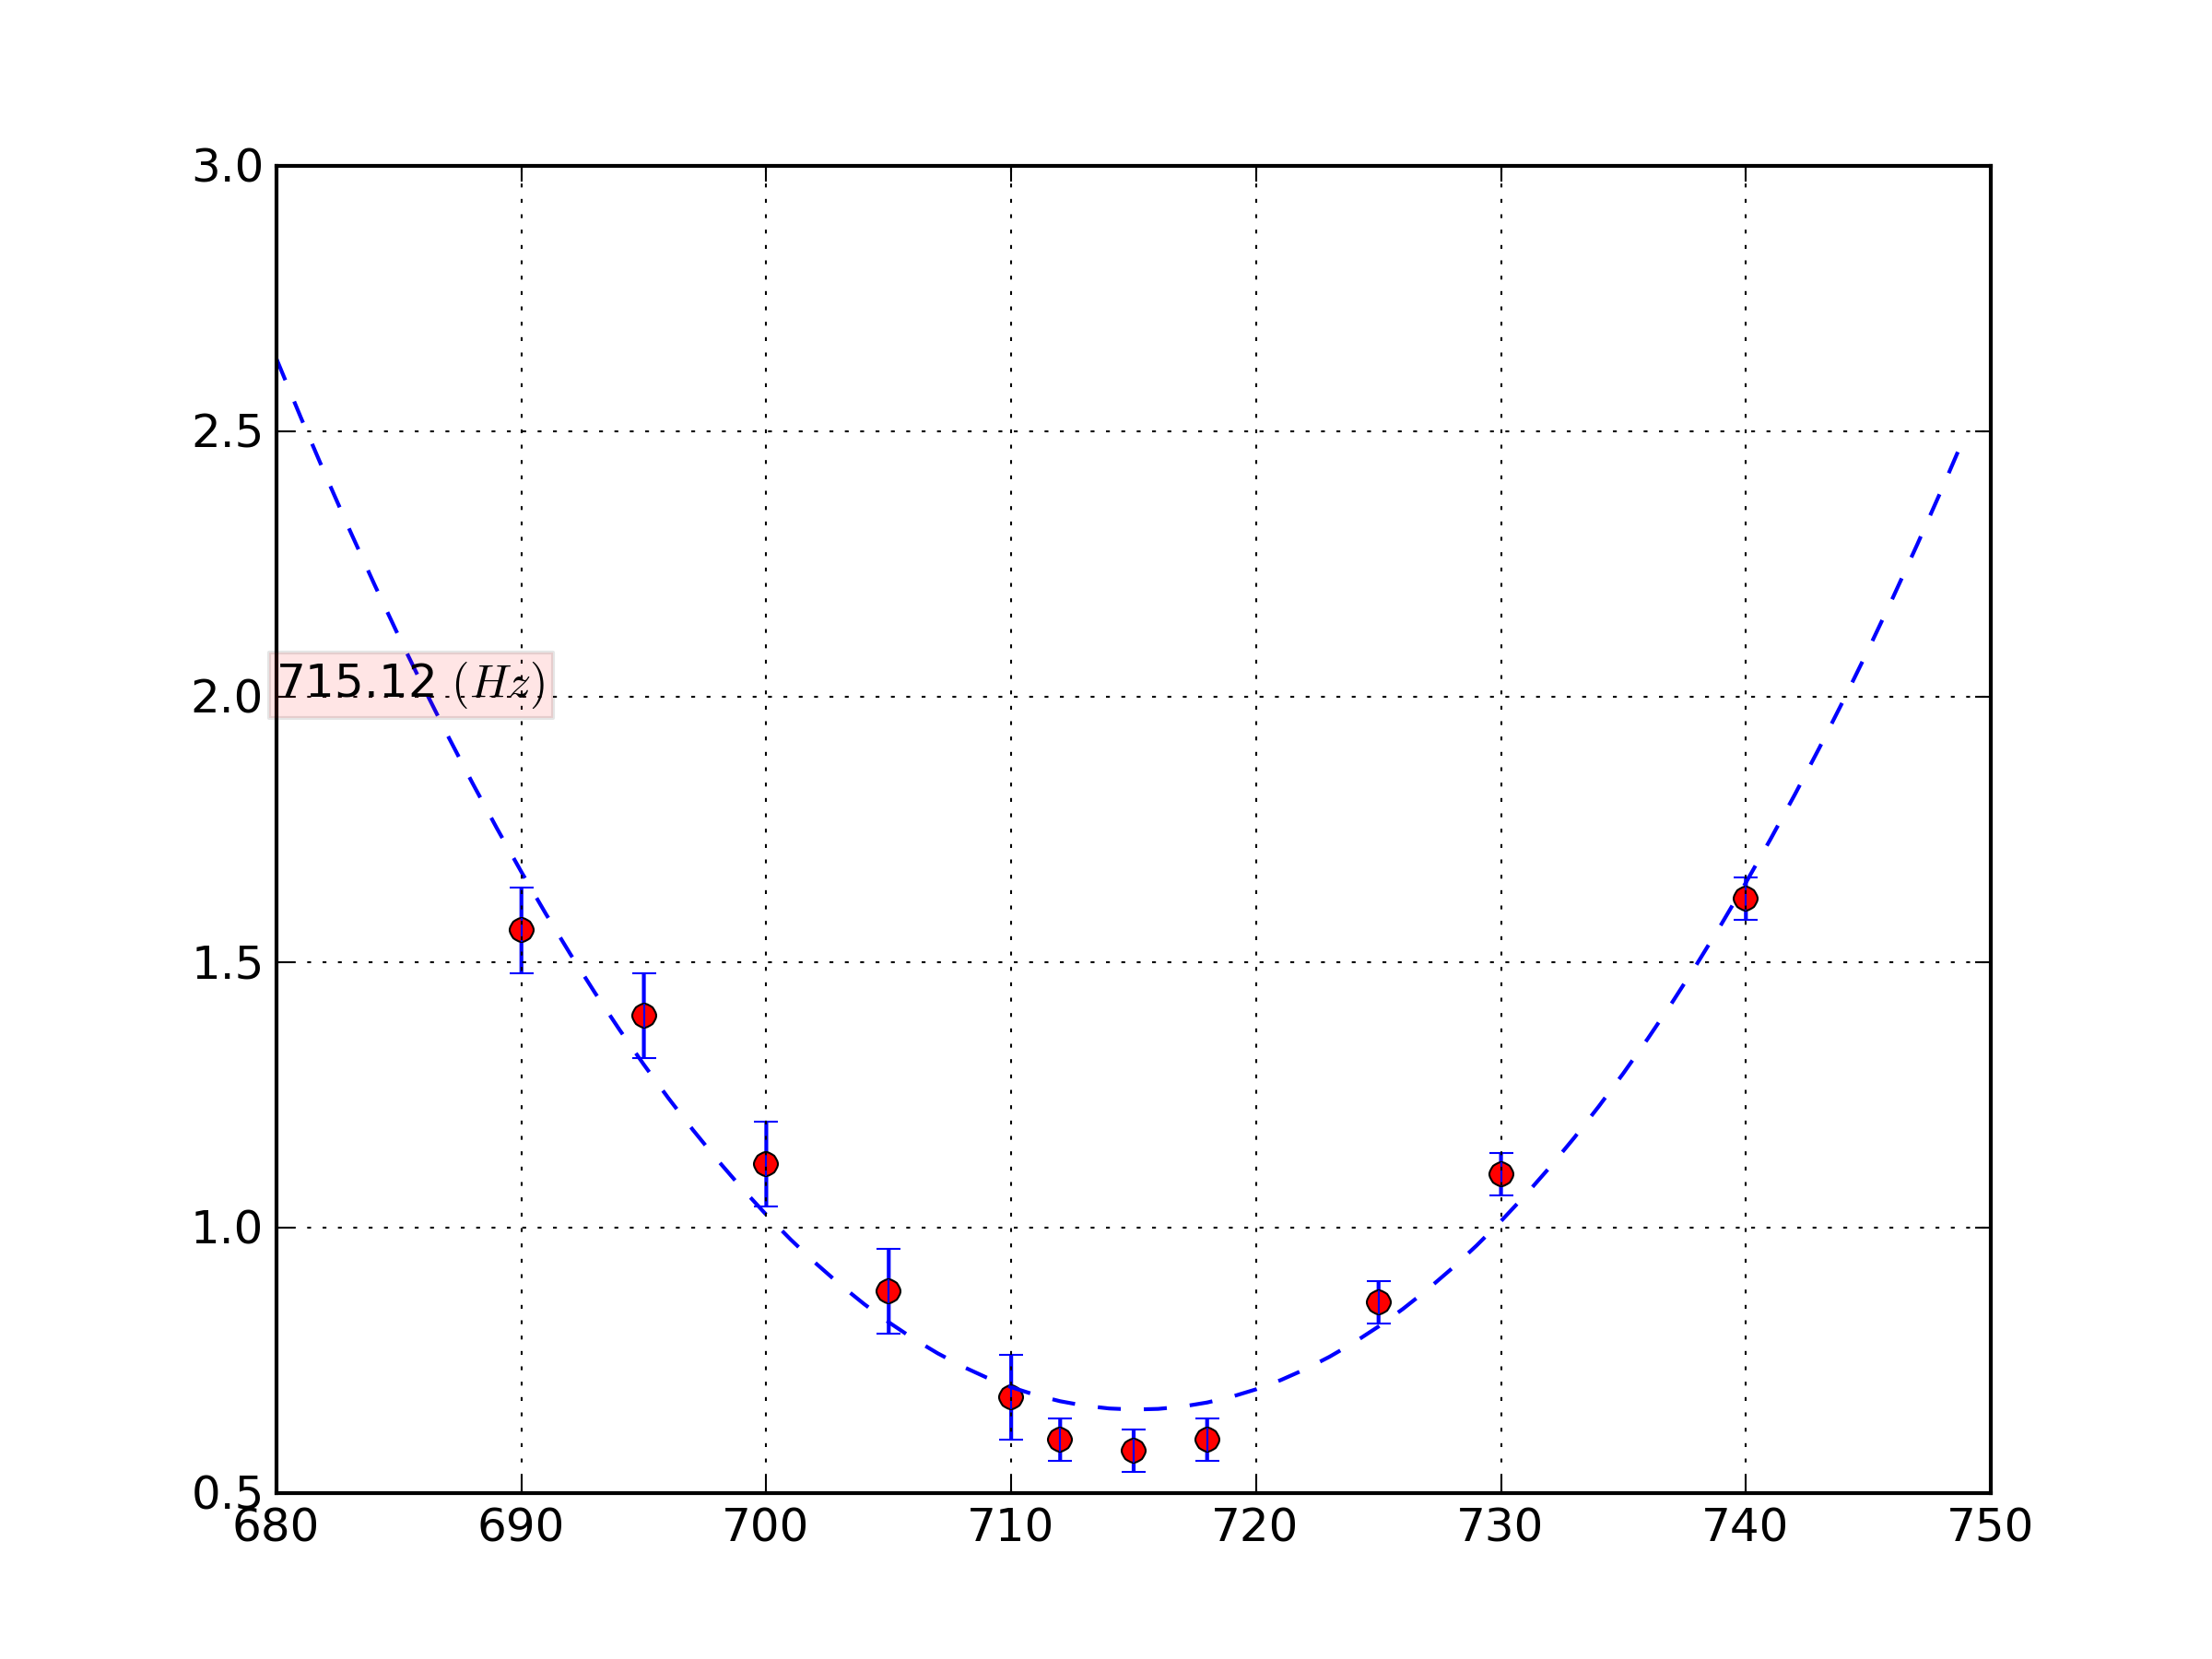
\includegraphics[scale=0.75]{grafici/EM/34.png}

\subparagraph*{l=32 cm}

\begin{sagesilent}
 #Fit per stimare i parametri -> Frequenza di risonanza: -b/2a

#Carico file
raw = np.recfromcsv('dati/EM/par32.csv')

#Seleziono dati per il fit
batch1 = raw[raw['freq']>700]
batch2 = batch1[batch1['freq']< 760]

#Carico negli array i dati giusti
freq = batch2['freq']
volt = batch2['vout']
yerr = batch2['errv']


def funz(x,a,b,c):
    return a*x^2+b*x+c

def func(P,x):
    return funz(x,P[0],P[1],P[2])

mymod = odr.Model(func)
mydata = odr.RealData(freq,volt)
myfit = odr.ODR(mydata,mymod,beta0=[1.,1.,1.],maxit=1000)
myout = myfit.run()

plt.clf()
xin = np.arange(min(freq)-10,max(freq)+10,1)
yin = func(myout.beta,xin)
plt.plot(freq,volt,'ro')
plt.errorbar(freq,volt,yerr,np.zeros_like(yerr),fmt=None)
plt.plot(xin,yin,'b--')
plt.grid(True)
myout.pprint()

#trovo minimo dai parametri x=-b/2*a
min4 = -myout.beta[1]/(2*myout.beta[0]) 
sd4 = sqrt(myout.sd_beta[1]**2/(2*myout.beta[0])**2 +(myout.beta[1]*myout.sd_beta[0])**2)/(2*myout.beta[0]**4)
#stampo minimo su grafico
s = repr(round(min4,2))+" $(KHz)$"
plt.text(725,1.6,s,fontsize=12,bbox=dict(facecolor='red',alpha=0.1))
print sd4
plt.savefig("grafici/EM/32.png",dpi=300)
\end{sagesilent}

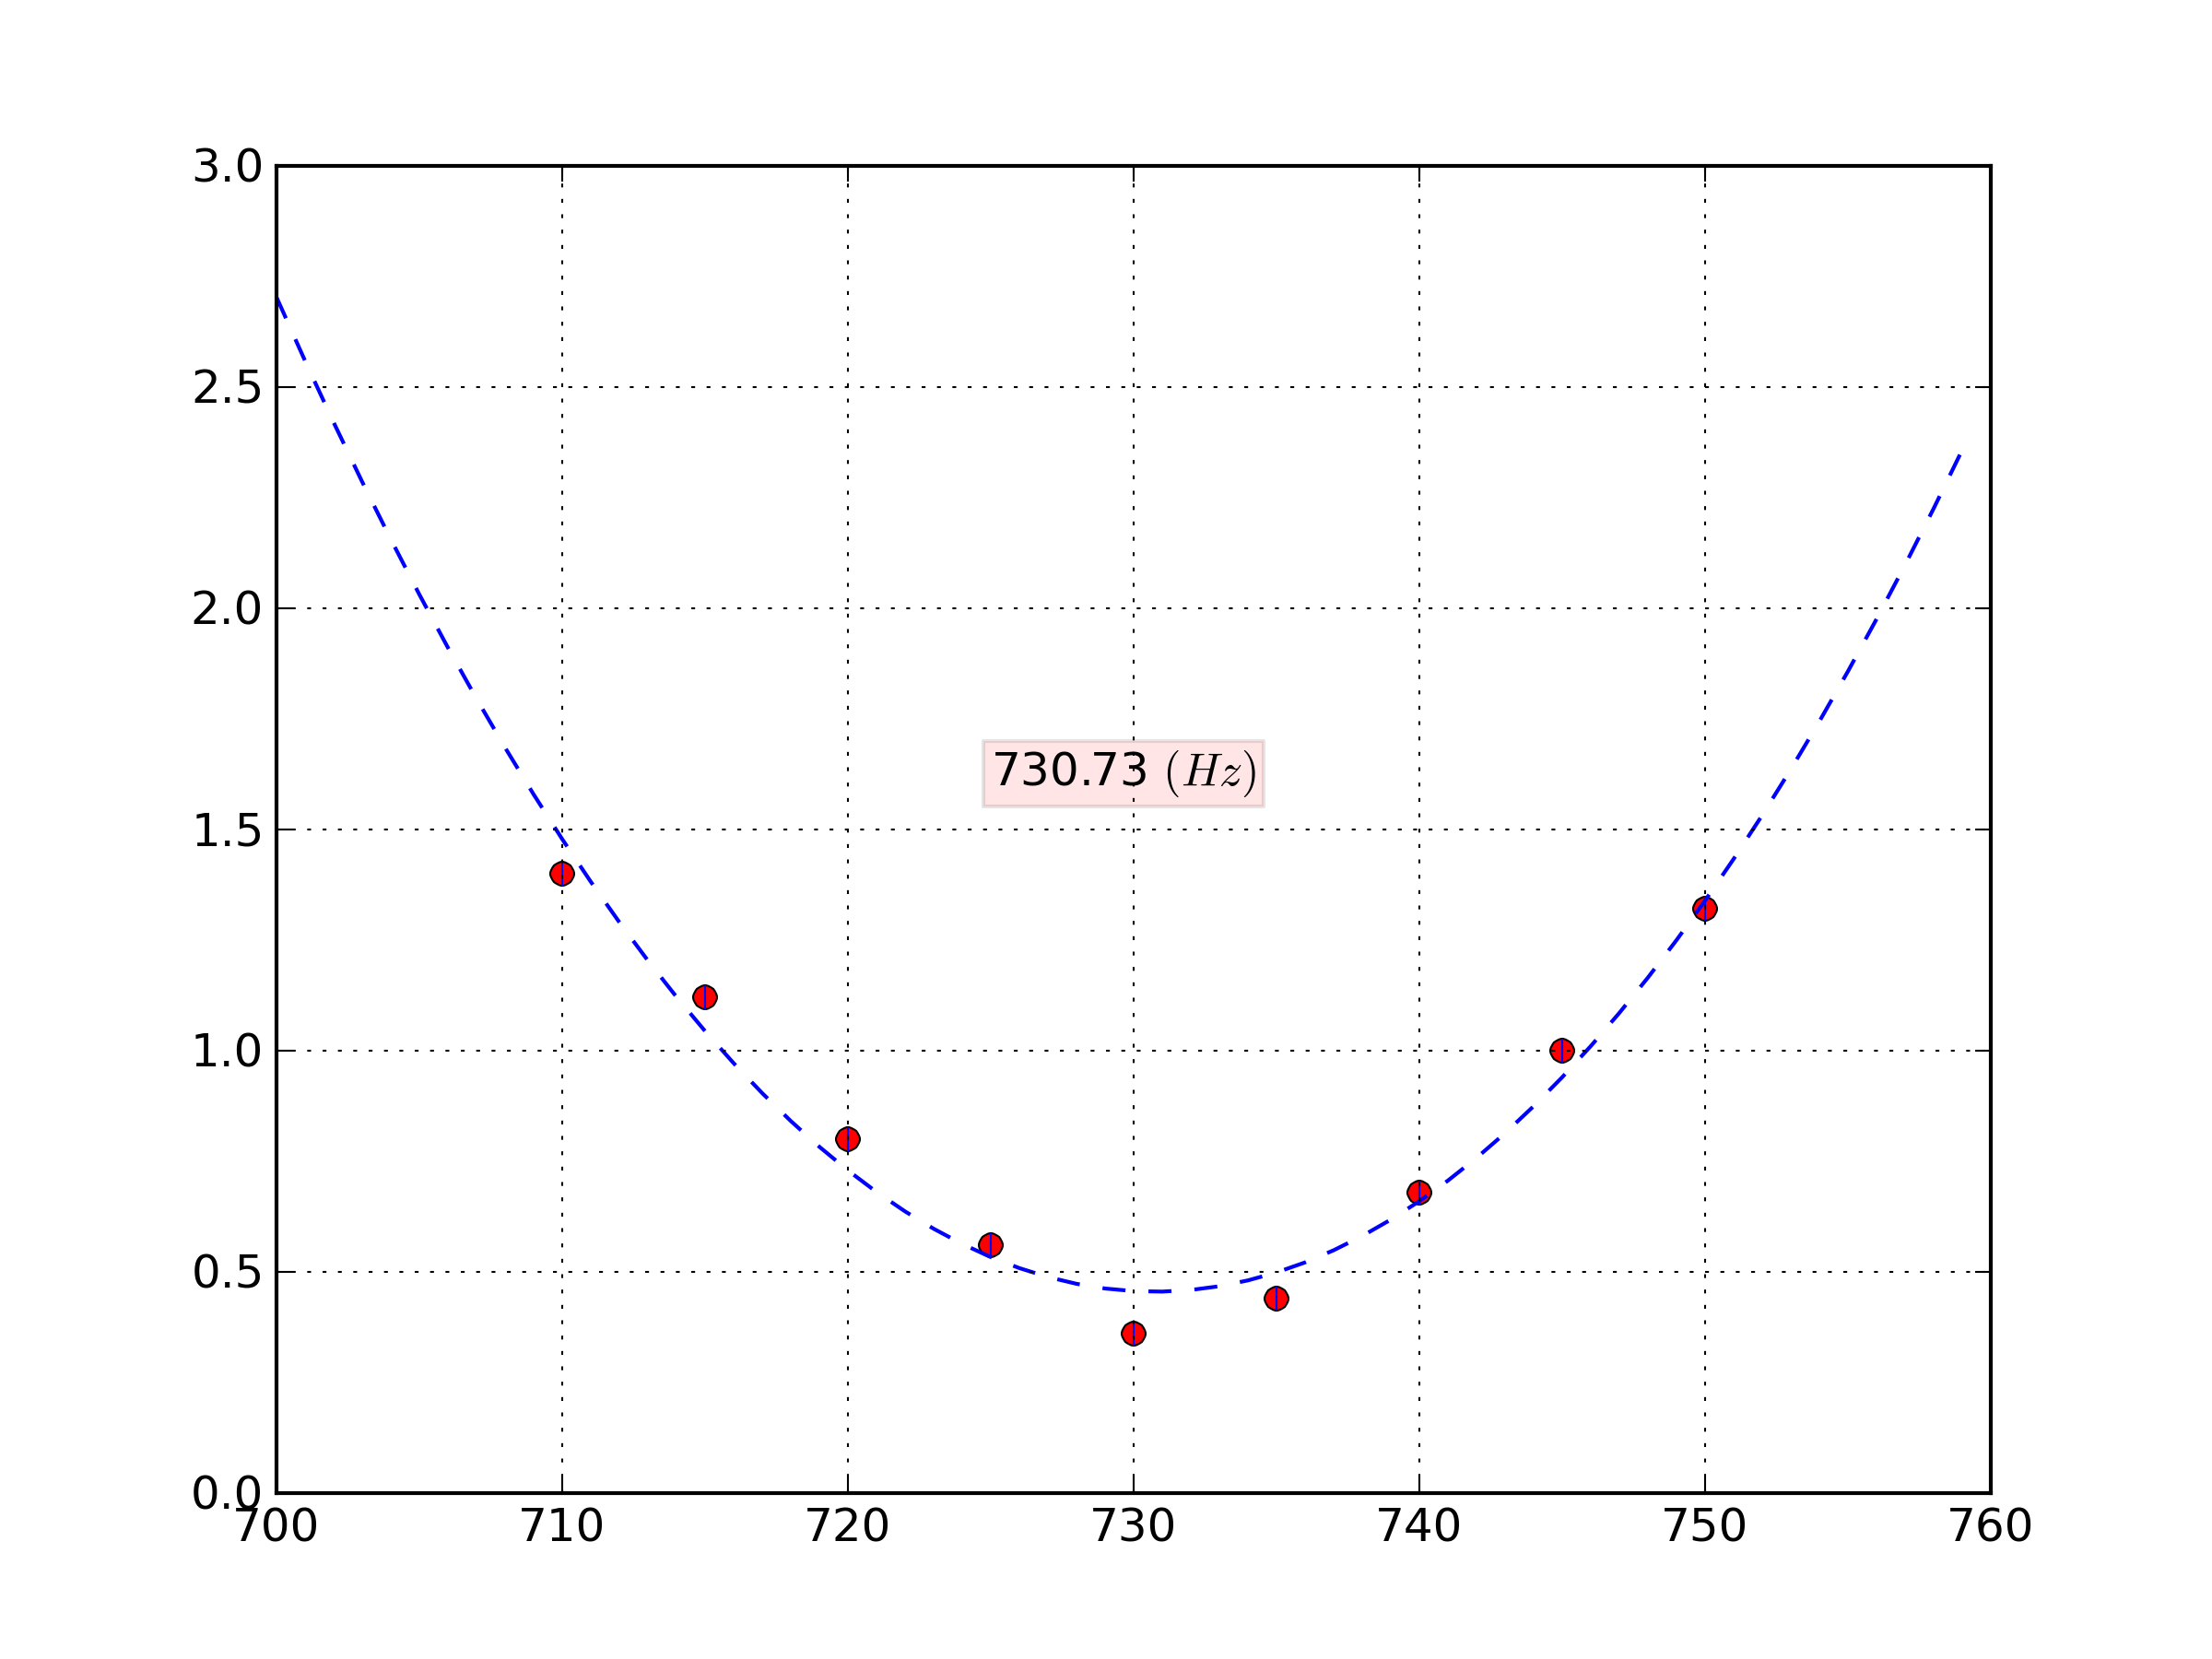
\includegraphics[scale=0.75]{grafici/EM/32.png}

\subparagraph*{l=28 cm}

\begin{sagesilent}
 #Fit per stimare i parametri -> Frequenza di risonanza: -b/2a

#Carico file
raw = np.recfromcsv('dati/EM/par28.csv')

#Seleziono dati per il fit
batch1 = raw[raw['freq']>740]
batch2 = batch1[batch1['freq']<800]

#Carico negli array i dati giusti
freq = batch2['freq']
volt = batch2['vout']
yerr = batch2['errv']


def funz(x,a,b,c):
    return a*x^2+b*x+c

def func(P,x):
    return funz(x,P[0],P[1],P[2])

mymod = odr.Model(func)
mydata = odr.RealData(freq,volt)
myfit = odr.ODR(mydata,mymod,beta0=[1.,1.,1.],maxit=1000)
myout = myfit.run()

plt.clf()
xin = np.arange(min(freq)-10,max(freq)+10,1)
yin = func(myout.beta,xin)
plt.plot(freq,volt,'ro')
plt.errorbar(freq,volt,yerr,np.zeros_like(yerr),fmt=None)
plt.plot(xin,yin,'b--')
plt.grid(True)

#trovo minimo dai parametri x=-b/2*a
min5 = -myout.beta[1]/(2*myout.beta[0]) 

#stampo minimo su grafico
s = repr(round(min5,2))+" $(KHz)$"
plt.text(765,1.5,s,fontsize=12,bbox=dict(facecolor='red',alpha=0.1))

plt.savefig("grafici/EM/28.png",dpi=300)
\end{sagesilent}



\includegraphics[scale=0.75]{grafici/EM/28.png}

\subsection*{Calcolo di c}

A questo punto fittiamo i valori di $\omega$ raccolti al variare di $l$, lunghezza del condensatore, per ricavare $c$ secondo la relazione:
\begin{equation}
 LC =\displaystyle \frac{1}{{\omega}^2} = l_c \cdot \epsilon_{0}\cdot \mu_{0}\cdot \frac{N^2 \cdot h \cdot log(\frac{R_{int}}{R_{ext}})}{log (\frac{b}{a})}
\end{equation}

Dove m è il coefficente angolare della retta. Nella funzione q rappresenta le capacità parassite presenti nel sistema e supposte in parallelo. Infatti:
$$L(C+C_p) = \frac{1}{\omega^2}$$

Prendiamo $y = \omega^{-2}$ e $x=l_c$, linearizzando quindi il nostro problema. 

\begin{sagesilent}

#Fit per il calcolo di c

<<<<<<< HEAD
freq= [min1, min2, min3, min4, min5]
=======
freq=np.array([min1, min2, min3, min4, min5])*1000*2*n(pi)
#freq.astype(float)
>>>>>>> 4f323eb24e423b48e956e64d185d2b8f8c762276
#2.773/2.083
k = (339**2)*0.0225*(ln(0.0937/0.05)/ln(418/358))
elle=[0.40,0.38,0.34,0.32,0.28]

omegavar=1./(freq*1000*2*3.14)**2 

def funz(x,a,c):
    return a*x+c

def func(P,x):
    return funz(x,P[0],P[1])

mymod = odr.Model(func)
mydata = odr.RealData(elle,omegavar)
myfit = odr.ODR(mydata,mymod,beta0=[1.,1.,1.],maxit=1000)
myout = myfit.run()
myout.pprint()

plt.clf()
#np.arange crea un array. Le proprietà dell'array sono (valore_min,valore_massimo,passo). come valore min e #max gli passo i valori min e max di omegavar che è la nostra x. In questo modo la funzione sarà contenuta 

xin = np.arange(0.8*min(elle),max(elle)*1.2,0.01)
yin = func(myout.beta,xin)
plt.plot(elle,omegavar,'ro')
#plt.errorbar(,volt,yerr,np.zeros_like(yerr),fmt=None)
plt.plot(xin,yin,'b--')
plt.grid(True)
m = myout.beta[0]
c = sqrt(k/myout.beta[0])
er = sqrt(k)* m**(-3/2) * myout.sd_beta[0]  
erc = sqrt((1/0.0000264585)/(4*k*m) + er^2)
par = myout.beta[1]*2*n(pi)/(339^2*0.0225*ln(9.37/5))
plt.savefig("grafici/EM/misurac.png",dpi=300)

\end{sagesilent}

\includegraphics[scale=0.75]{grafici/EM/misurac.png}


Dal fit ricaviamo i seguenti valori:

$\sage{round(c,1)} \pm \sage{round(erc,1)}\ m \cdot s^{-1}$ 

L'errore è stato ricavato tramite la seguente formula di propagazione:
$\sigma_c = \frac{\sqrt(k)\sigma_m}{m^{3/2}}$

Per ricavare c, abbiamo diviso il coeff. angolare m per il coefficente geometrico k:
$$ k = \displaystyle \frac{N^2 \cdot h \cdot ln(R_e/R_i)}{ln(b/a)}$$

$c =\displaystyle \sqrt{\frac{k}{m}} = \sqrt{\frac{1}{\mu_0 \cdot \epsilon_0 }}$

Il valore della capacità parassita è $5.4\cdot 10^{-17} F$.
